\section{Teleskop}
Das verwendete Teleskop ist vom Typ \textsc{Cassegrain}, siehe Abb.\ (\ref{fig:cassegrain}).
\begin{figure}[t]
  \centering
  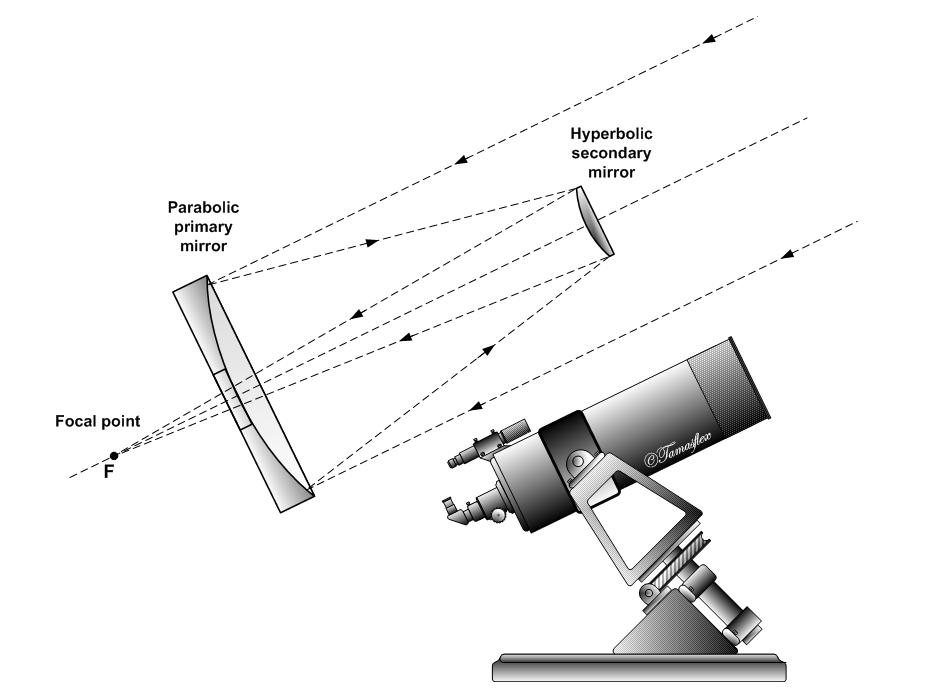
\includegraphics[width=.5\textwidth]{Cassegrain.en.png}
  \caption{Schematische Darstellung eines \textsc{Cassegrain}--Teleskops.\cite{wikipediaCassegrain}} \label{fig:cassegrain}
\end{figure}
Mit Hilfe der Software \textit{Cartes du Ciel}, können Sterne am Himmel ausgewählt werden und dann mit der Software \textit{N.I.N.A} vom Teleskop angefahren werden.
Mit dem Okular kann der Stern beobachtet werden und per Fernbedienung wird das Teleskop so ausgerichtet, dass der Stern genau mittig im Okular zu sehen ist.
